\documentclass[a4paper, 11pt]{article}

\usepackage[T1]{fontenc}
\usepackage[utf8]{inputenc}
\usepackage[italian]{babel}
\usepackage{geometry}
\geometry{a4paper, top=2cm, bottom=2cm, left=2cm, right=2cm}
\usepackage{enumitem}
\usepackage[table]{xcolor}
\usepackage{xcolor}
\usepackage{graphicx}
\usepackage{listings}
\usepackage{float}
\usepackage{color}
\usepackage{hyperref} % Da inserire nel preambolo


% --- Configurazione Grafica ---
\graphicspath{{./images/}} % Cartella dove salvare le tue immagini (opzionale)

% --- Configurazione Stile Codice Java ---
\definecolor{javagreen}{rgb}{0.25,0.5,0.35}
\definecolor{javapurple}{rgb}{0.5,0,0.35}
\definecolor{javablue}{rgb}{0,0,0.8}
\definecolor{javastring}{rgb}{0.6,0.1,0.1} % Definito colore mancante per le stringhe
\definecolor{bgcode}{rgb}{0.95,0.95,0.92}

% Colori specifici per SQL (puoi usare anche quelli che hai già definito)
\definecolor{sqlblue}{RGB}{0,0,180}
\definecolor{sqlgreen}{RGB}{34,139,34}
\definecolor{sqlgray}{RGB}{100,100,100}

% Nuovo stile per SQL
\lstdefinestyle{stileSQL}{
	language=SQL,
	basicstyle=\ttfamily\small,
	keywordstyle=\color{sqlblue}\bfseries,
	stringstyle=\color{sqlgreen},
	commentstyle=\color{sqlgray}\itshape,
	numbers=none,
	tabsize=4,
	showspaces=false,
	showstringspaces=false,
	breaklines=true,
	frame=single,
	xleftmargin=-10pt, % Mantiene lo spostamento a sinistra che hai chiesto prima
	morekeywords={SELECT,INSERT,UPDATE,DELETE,FROM,WHERE,AND,OR,LIMIT} % Keyword extra se servono
}


\lstset{
	language=Java,
	basicstyle=\ttfamily\small,
	keywordstyle=\color{javablue}\bfseries,
	stringstyle=\color{javastring},      % Corretto da javachr a javastring
	commentstyle=\color{javagreen}\itshape,
	morecomment=[s][\color{javapurple}]{/**}{*/},
	numbers=none,                 % Numeri di riga a sinistra
	numberstyle=\tiny\color{gray},
	stepnumber=1,
	numbersep=10pt,
	tabsize=4,
	showspaces=false,
	showstringspaces=false,
	breaklines=true,              % Va a capo automaticamente
	frame=single                  % Bordo intorno al codice
}


\title{Weather Station
\\Software per servizi metereologici}
\author{Giulio Nencini - MAT: 7115972
\\Yuri Bartoletti - MAT: 7113273}
\date{\today}

\begin{document}
	\newpage
	\maketitle
	\tableofcontents

	\newpage
	\section{Presentazione del progetto}
	\subsection{Statement}
	Il software sviluppato è un sistema composto principalmente da due parti: misurazione di alcune grandezze fisiche meteorologiche ad opera di alcuni sensori, tali misurazioni saranno visibili dagli utenti che desidereranno vederle, e sistema di notificazione agli utenti iscritti qualora una di queste misurazioni dovesse violare dei limiti impostati nelle "AlertRule" dall'utente stesso. Vi è inoltre un sistema interno che si occupa della sorveglianza dei sensori: qualora si dovessero riscontrare misurazioni anomale scatterà l'apertura di un ticket e ci sarà un manutentore che provvederà alla riparazione o alla sostituzione del sensore guasto.

	\subsection{Pratiche e ambienti di sviluppo}
	Il software è stato interamente sviluppato in Java, mentre per il database è stato usato PostgreSQL mediante la libreria JBDC. Tutti i diagrammi sono stati realizzati con Gaphor, tranne il modello relazionale che è stato realizzato mediante il sito DrawSQL.app e il navigation diagram che è stato realizzato con draw.io.
	Per quanto riguarda la progettazione, abbiamo optato per la separazione del software in tre diversi package:
	\begin{itemize}
		\item \textbf{Business Logic}: per le classi che implementano la logica di business del sistema.
		\item \textbf{Domain Model}: contiene le classi che rappresentano le entità del sistema.
		\item \textbf{ORM}: contiene le classi che implementano l’Object-Relational Mapping, fondamentale al fine di rendere i dati permanenti in un db.
	\end{itemize}
	Per poter interagire col software è stata creata un'interfaccia a riga di comando.
	\\
	Il codice è presente al seguente repo di GitHub: \url{https://github.com/Yuri0303/Weather_Station_SWE}
	\\
	Durante lo sviluppo di questo progetto è stato fatto uso di intelligenza artificiale generativa per debug, suggerimenti su cosa fosse meglio fare per alcune cose e aiuto nella ricerca di funzionalità utili ai nostri fini. Il modello usato è GeminiPro.
	\\
	Prima di passare alla presentazione delle varie classi, ecco di seguito il Dependency Package Diagram, che illustra dove i vari package fanno uso di metodi esterni:
	\begin{figure}[H]
		\centering
		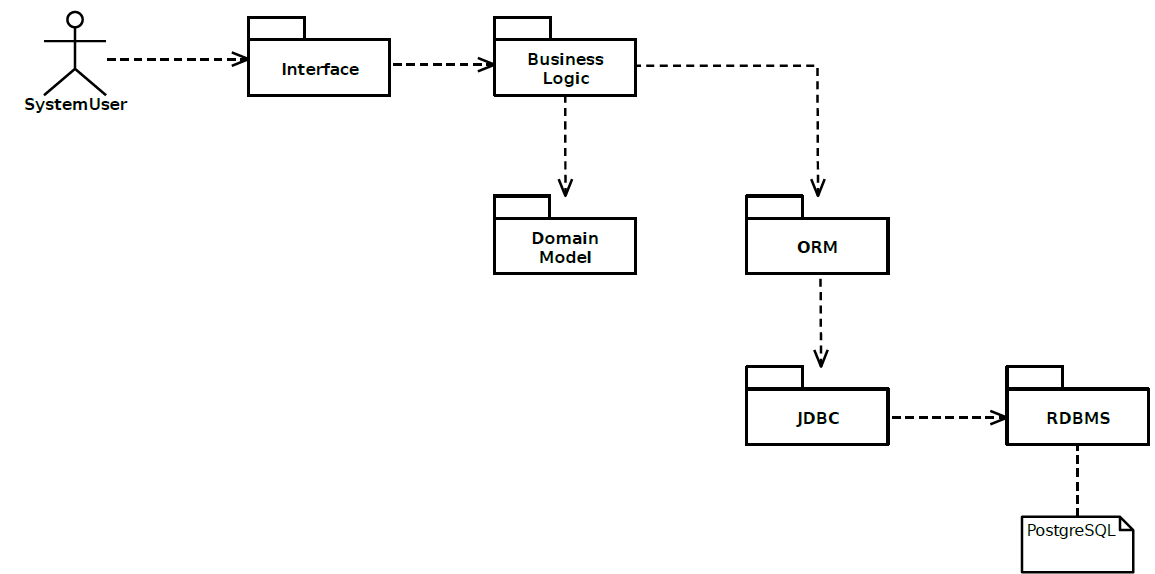
\includegraphics[width=0.95\textwidth]{Images/package_dependencies}
		\caption{Package Dependencies}
		\label{fig:package_dependecies}
	\end{figure}

	\section{Progettazione}
	\subsection{Use Case Diagram}
	L'attore \textbf{User} è il cliente utilizzatore dei servizi del software, può di base leggere le misurazioni effettuate oppure impostare una alert rule. \textbf{L'Admin} svolge l'esecizio di sorveglianza manuale del corretto funzionamento dei sensori, così come quello di amministratore generale del sistema, è l'unica entità che può bloccare un utente. Il \textbf{SystemMonitor} svolge una sorveglianza automatica (periodica) in merito al corretto funzionamento dei sensori. Sia quest'ultimo che l'admin possono aprire dei ticket in seguito al riscontro di un'anomalia, ticket che sarà preso da uno dei \textbf{Maintainer}, che interverrà sul sensore segnalato riparandolo o sostituendolo.
	\begin{figure}[H]
		\centering
		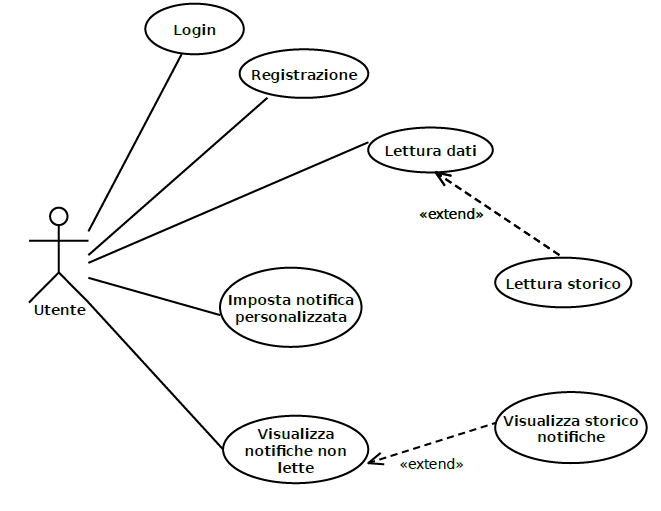
\includegraphics[width=0.95\textwidth]{Images/use_cases_User}
		\caption{Use Cases User}
		\label{fig:use_uase_User}
	\end{figure}
	\begin{figure}[H]
		\centering
		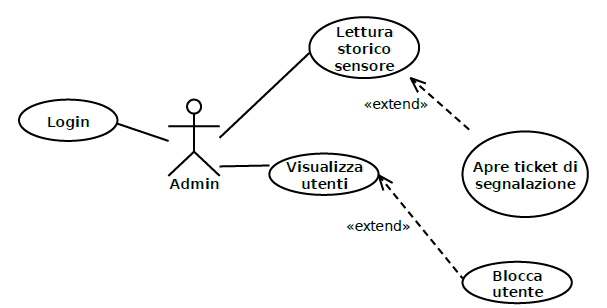
\includegraphics[width=0.95\textwidth]{Images/use_cases_Admin}
		\caption{Use Case Admin}
		\label{fig:use_case_Admin}
	\end{figure}
	\begin{figure}[H]
		\centering
		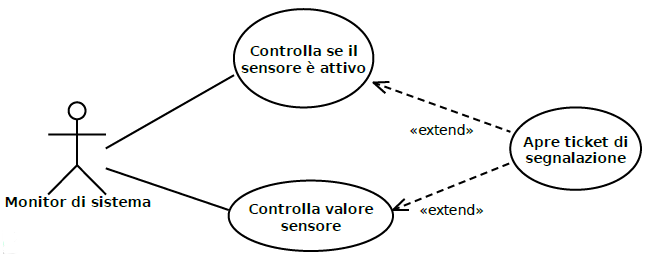
\includegraphics[width=0.95\textwidth]{Images/use_cases_SystemMonitor}
		\caption{Use Case SystemMonitor}
		\label{fig:use_caseSystemMonitor}
	\end{figure}
	\begin{figure}[H]
		\centering
		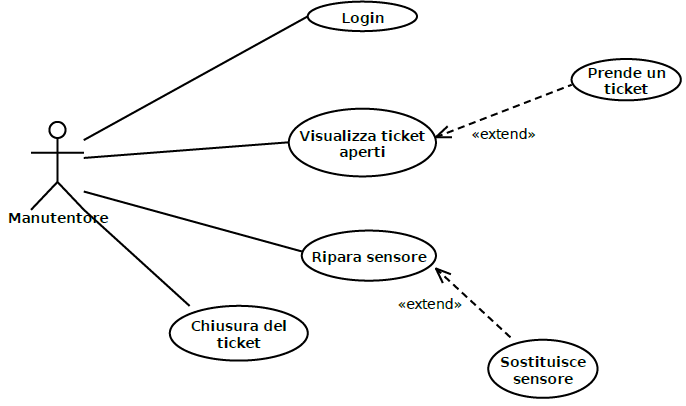
\includegraphics[width=0.95\textwidth]{Images/use_cases_Maintainer}
		\caption{Use Case Maintainer}
		\label{fig:use_case_Maintainer}
	\end{figure}

	\newpage
	\subsection{Use Case Template}
%=========================================================================================================================================
%\input{UsecaseTemplate}


	\begin{table}[h]
		\centering
		\setlength{\arrayrulewidth}{0.8pt} % Raddoppia lo spessore delle linee
		% Attiva l'alternanza colori dalla riga 2
		\rowcolors{2}{white}{blue!10}

		% Definizione con un solo | per il bordo sinistro e destro
		\begin{tabular}{|l p{12cm}|}
			\hline % Bordo superiore

			\rowcolor{gray!25}
			\textbf{Use Case \#1} & \textbf{Accedi al sistema (Sign-in)} \\
			\textbf{Brief Description} & L'utente del sistema accede usando le proprie credenziali\\
			\textbf{Level} & User Goal \\
			\textbf{Actors} & User, Admin, Maintainer \\
			\textbf{Pre-Conditions} & L'utente di sistema deve essere sulla pagina dedicata all'accesso \\ %(mockup)
			\textbf{Basic Flow} & \begin{enumerate}[label=\arabic*), leftmargin=*, before=\vspace{-0.7cm}, after=\vspace{-0.4cm}]
									  \item L'utente di sistema seleziona la propria pagina di login
									  \item L'utente inserisce le proprie credenziali
									  \item L'utente invia le proprie credenziali
									  \item Il sistema verifica le credenziali
									  \item Il sistema autentica l'utente
									  \item[]
			\end{enumerate} \\
			\textbf{Alternative Flow} & 4.a) Se le credenziali sono errate, l'utente non è registrato oppure è sulla pagina di login errata, il sistema restituisce un messaggio di errore e permette di ritentare \\ %(test)
			\textbf{Post-Conditions} & L'utente è autenticato nel sistema e ha accesso alle sue funzioni \\

			\hline % Bordo inferiore
		\end{tabular}

		\vspace{0.2cm}
		\caption{Use Case \#1 (Accedi al sistema)}
	\end{table}

	\vspace{1cm}

	\begin{table}[h]
		\centering
		\setlength{\arrayrulewidth}{0.8pt} % Raddoppia lo spessore delle linee
		\rowcolors{2}{white}{blue!10}

		\begin{tabular}{|l p{12cm}|}
			\hline

			\rowcolor{gray!25}
			\textbf{Use Case \#2} & \textbf{Registrazione (Sing-Up)} \\
			\textbf{Brief Description} & L'utente si registra creando un nuovo account \\
			\textbf{Level} & User Goal \\
			\textbf{Actors} & User \\
			\textbf{Pre-Conditions} & L'utente deve essere nella pagina di registrazione \\ %(mockup)
			\textbf{Basic Flow} & \begin{enumerate}[label=\arabic*), leftmargin=*, before=\vspace{-0.7cm}, after=\vspace{-0.4cm}]
									  \item L'utente  fornisce le informazioni richieste
									  \item l'utente conferma la registrazione
									  \item Il sistema verifica i dati (email ha vincolo unique)
									  \item Il sistema crea un nuovo account per il cliente
									  \item[]
			\end{enumerate} \\
			\textbf{Alternative Flow} & 3.a) Se i dati non sono validi o sono già presenti in un altro account, il sistema mostra un messaggio di errore e permette di ritentare\\
			\textbf{Post-Conditions} & Il sistema mostra il messaggio dell'avvenuta registrazione e riporta l'utente nella pagina di login \\

			\hline
		\end{tabular}

		\vspace{0.2cm}
		\caption{Use Case \#2 (Registrati al sistema)}
	\end{table}

	\vspace{1cm}

	\begin{table}[h]
		\centering
		\setlength{\arrayrulewidth}{0.8pt} % Raddoppia lo spessore delle linee
		\rowcolors{2}{white}{blue!10}

		\begin{tabular}{|l p{12cm}|}
			\hline

			\rowcolor{gray!25}
			\textbf{Use Case \#3} & \textbf{Apertura del ticket (Admin)} \\
			\textbf{Brief Description} & L'Admin apre una segnalazione su un sensore \\
			\textbf{Level} & User Goal\\
			\textbf{Actors} & Admin \\
			\textbf{Pre-Conditions} & L'Admin deve aver fatto l'accesso e deve essere sulla pagina di "Lettura storico" \\
			\textbf{Basic Flow} & \begin{enumerate}[label=\arabic*), leftmargin=*, before=\vspace{-0.7cm}, after=\vspace{-0.4cm}]
									  \item L'Admin seleziona l'opzione "Segnala sensore"
									  \item L'Admin seleziona il sensore da segnalare
									  \item Il sistema registra il ticket sul sensore segnalato
									  \item[]
			\end{enumerate} \\
			% \textbf{Alternative Flow} & \\
			\textbf{Post-Conditions} & Il ticket è stato registrato. Il sistema blocca il sensore segnalato e riporta l'Admin sulla pagina di "Lettura storico", così, se necessario, può aprire subito un altro ticket \\

			\hline
		\end{tabular}

		\vspace{0.2cm}
		\caption{Use Case \#3 (Admin: Apri ticket)}
	\end{table}
	\vspace{1cm}

	\begin{table}[h]
		\centering
		\setlength{\arrayrulewidth}{0.8pt} % Raddoppia lo spessore delle linee
		\rowcolors{2}{white}{blue!10}

		\begin{tabular}{|l p{12cm}|}
			\hline

			\rowcolor{gray!25}
			\textbf{Use Case \#4} & \textbf{Apertura del ticket (Monitor di Sistema)} \\
			\textbf{Brief Description} & Il Monitor di Sistema apre una segnalazione su un sensore \\
			\textbf{Level} & System Goal\\
			\textbf{Actors} & SystemMonitor \\
			\textbf{Pre-Conditions} & Il Monitor di Sistema è "sveglio" \\
			\textbf{Basic Flow} & \begin{enumerate}[label=\arabic*), leftmargin=*, before=\vspace{-0.7cm}, after=\vspace{-0.4cm}]
									  \item Il Monitor verifica se ci sono anomalie nei sensori: verifica se l'ultima lettura dei sensori è in un range valido
									  \item Il sistema registra il ticket sul sensore anomalo
									  \item[]
			\end{enumerate} \\
			\textbf{Alternative Flow} & 2.a) Il sistema non registra alcun ticket perché il Monitor non ha rilevato anomalie \\
			\textbf{Post-Conditions} & Il sistema ha correttamente registrato il ticket (se è stato creato) e ha bloccato il sensore guasto\\

			\hline
		\end{tabular}

		\vspace{0.2cm}
		\caption{Use Case \#4 (SystemMonitor: Apri ticket)}
	\end{table}
	\vspace{1cm}

	\begin{table}[h]
		\centering
		\setlength{\arrayrulewidth}{0.8pt} % Raddoppia lo spessore delle linee
		\rowcolors{2}{white}{blue!10}

		\begin{tabular}{|l p{12cm}|}
			\hline

			\rowcolor{gray!25}
			\textbf{Use Case \#5} & \textbf{Prendere un ticket} \\
			\textbf{Brief Description} & Il manutentore prende un ticket aperto\\
			\textbf{Level} & User Goal \\
			\textbf{Actors} & Maintainer \\
			\textbf{Pre-Conditions} & Il manutentore deve essere autenticato e nella pagina "Visualizza ticket aperti". Inoltre, non deve avere già preso un ticket \\
			\textbf{Basic Flow} & \begin{enumerate}[label=\arabic*), leftmargin=*, before=\vspace{-0.7cm}, after=\vspace{-0.4cm}]
									  \item Il manutentore seleziona l'opzione "Prendi ticket"
									  \item Il manutentore seleziona il ticket che vuole prendere
									  \item Il sistema registra il ticket come preso
									  \item[]
			\end{enumerate} \\
			\textbf{Alternative Flow} & 3.a) Il sistema segnala un errore perché il ticket selezionato è già stato acquisito da un altro manutentore qualche istante prima\\
			\textbf{Post-Conditions} & Il sistema imposta il ticket come "preso" \\

			\hline
		\end{tabular}

		\vspace{0.2cm}
		\caption{Use Case \#5 (Prendi un ticket)}
	\end{table}

	\begin{table}[h]
		\centering
		\setlength{\arrayrulewidth}{0.8pt} % Raddoppia lo spessore delle linee
		\rowcolors{2}{white}{blue!10}

		\begin{tabular}{|l p{12cm}|}
			\hline

			\rowcolor{gray!25}
			\textbf{Use Case \#6} & \textbf{Riparazione di un sensore} \\
			\textbf{Brief Description} & Un manutentore che ha preso un ticket procede a riparare il sensore \\
			\textbf{Level} & User Goal \\
			\textbf{Actors} & Maintainer \\
			\textbf{Pre-Conditions} & Il manutentore è autenticato e ha già preso un ticket \\
			\textbf{Basic Flow} & \begin{enumerate}[label=\arabic*), leftmargin=*, before=\vspace{-0.7cm}, after=\vspace{-0.4cm}]
									  \item Il manutentore ripara il sensore
									  \begin{enumerate}[label=\arabic*), leftmargin=*, before=\vspace{-0.3cm}, after=\vspace{-0.3cm}]
										  \item[1.a)] Il manutentore reimposta lo stato del sensore come "attivo"
									  \end{enumerate}
									  \item Il manutentore chiude il ticket
									  \item[]
			\end{enumerate} \\
			\textbf{Alternative Flow} & \begin{enumerate}[label=\arabic*), before=\vspace{-0.7cm}, after=\vspace{-0.4cm}]
											\item[1.bis)] Il manutentore sostituisce il sensore se non riesce a ripararlo
											\begin{enumerate}[label=\arabic*), leftmargin=*, before=\vspace{-0.3cm}, after=\vspace{-0.3cm}]
												\item[1.bis.a)] Il manutentore imposta lo stato del sensore a "disattivato"
												\item[1.bis.b)] Il manutentore registra un nuovo sensore dello stesso tipo di quello sostituito
												\item[]
											\end{enumerate}
			\end{enumerate} \\
			\textbf{Post-Conditions} & Il sensore è stato riattivato oppure è stato disattivato definitivamente e sostituito\\

			\hline
		\end{tabular}

		\vspace{0.2cm}
		\caption{Use Case \#6 (Ripara sensore)}
	\end{table}
	\vspace{1cm}

	\begin{table}[h]
		\centering
		\setlength{\arrayrulewidth}{0.8pt} % Raddoppia lo spessore delle linee
		\rowcolors{2}{white}{blue!10}

		\begin{tabular}{|l p{12cm}|}
			\hline

			\rowcolor{gray!25}
			\textbf{Use Case \#7} & \textbf{Lettura dello storico dei dati (User)} \\
			\textbf{Brief Description} & L'utente legge le misurazioni dei sensori effettuate fino a una certa quantità di giorni precedenti alla data odierna \\
			\textbf{Level} & User Goal \\
			\textbf{Actors} & User \\
			\textbf{Pre-Conditions} & L'utente è autenticato e sulla pagina di lettura dati \\
			\textbf{Basic Flow} & \begin{enumerate}[label=\arabic*), leftmargin=*, before=\vspace{-0.7cm}, after=\vspace{-0.4cm}]
									  \item L'utente seleziona l'opzione "Leggi storico"
									  \item L'utente inserisce il numero di giorni di cui vuole leggere le misurazioni
									  \item Il sistema mostra tutte le misurazioni fatte da tutti i sensori in quell'arco di tempo
									  \item[]
			\end{enumerate} \\
			\textbf{Alternative Flow} & 3.a) Il sistema mostra un errore se il numero di giorni inserito non è valido ($\le$0 o troppo grande) \\
			\textbf{Post-Conditions} & Il sistema deve mostrare tutte e solo le misurazioni fatte in quell'arco di tempo \\

			\hline
		\end{tabular}

		\vspace{0.2cm}
		\caption{Use Case \#7 (User: Lettura storico)}
	\end{table}
	\vspace{1cm}

	\begin{table}[h]
		\centering
		\setlength{\arrayrulewidth}{0.8pt} % Raddoppia lo spessore delle linee
		\rowcolors{2}{white}{blue!10}

		\begin{tabular}{|l p{12cm}|}
			\hline

			\rowcolor{gray!25}
			\textbf{Use Case \#8} & \textbf{Impostare notifiche personalizzate} \\
			\textbf{Brief Description} &  L'utente crea una regola. Se qualsiasi sensore di quel tipo supera i limiti impostati, l'utente riceverà una notifica \\
			\textbf{Level} & User Goal \\
			\textbf{Actors} & User \\
			\textbf{Pre-Conditions} & L'utente è autenticato e sulla pagina principale \\
			\textbf{Basic Flow} & \begin{enumerate}[label=\arabic*), leftmargin=*, before=\vspace{-0.7cm}, after=\vspace{-0.4cm}]
									  \item L'utente seleziona l'opzione "Imposta alert rule personalizzata"
									  \item L'utente crea la regola impostando il tipo di sensore e i limiti inferiore e superiore. Il sistema verificherà automaticamente questa regola per ogni misurazione, ad opera dei sensori di quel tipo, successiva alla creazione
									  \item Il sistema registra la regola nel database
									  \item[]
			\end{enumerate} \\
			\textbf{Alternative Flow} & 3.a) Il sistema mostra un errore perché qualche valore della regola non è valido oppure se la regola esiste già \\
			\textbf{Post-Conditions} & L'utente rimane sulla pagina per impostare le notifiche personalizzate, qualora volesse impostarn un'altra \\

			\hline
		\end{tabular}

		\vspace{0.2cm}
		\caption{Use Case \#8 (Imposta notifica personalizzata)}
	\end{table}
	\vspace{1cm}

%==========================================================================================================================================================
	\clearpage
	\subsection{Class Diagram}
	\subsubsection{Domain Model}
	Contiene le entità del sistema, solo due di esse hanno al loro interno un metodo sfruttato da alcune classi della business logic. Per il resto sono solo classi di getter e setter, se non addirittura composte solo dal costruttore.
	\begin{figure}[H]
		\centering
		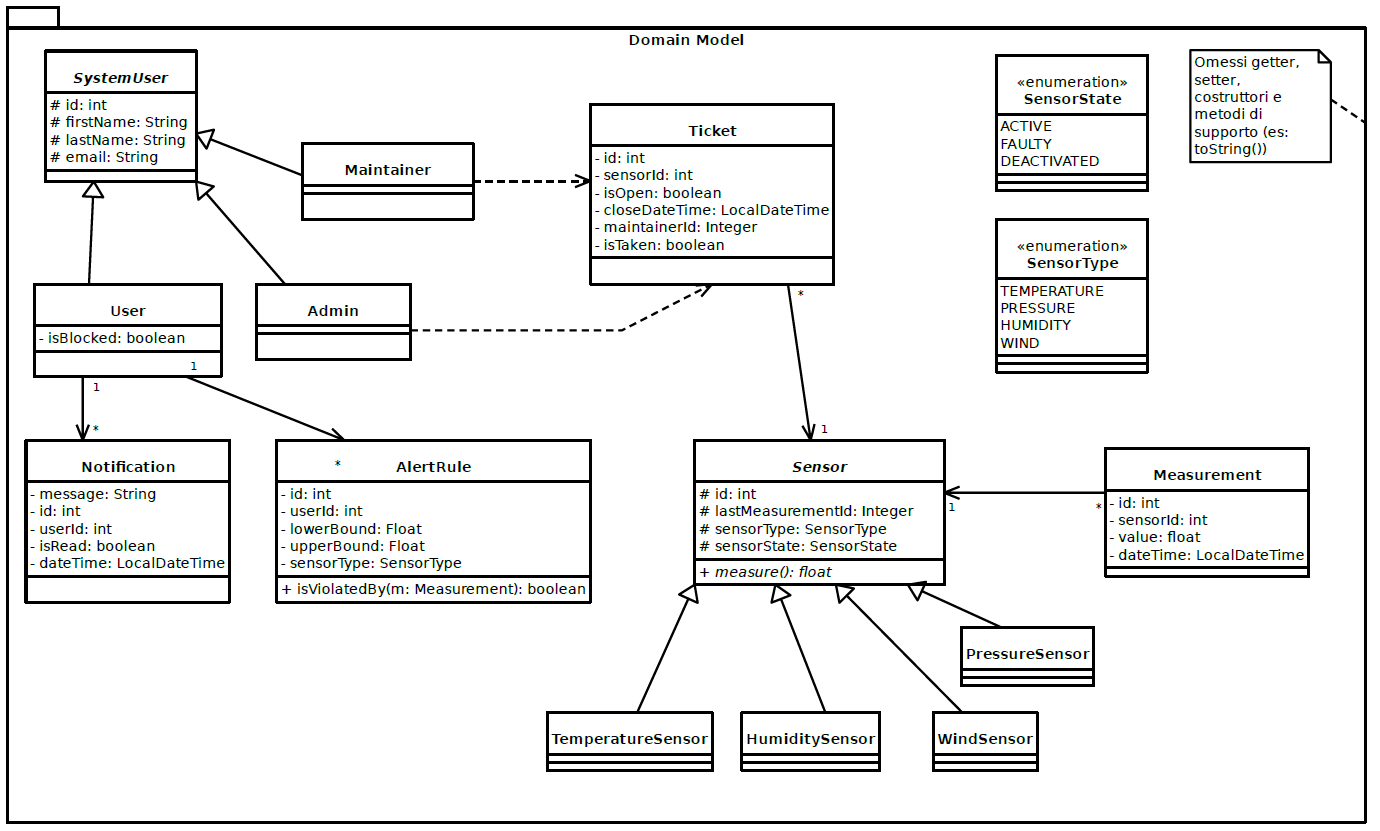
\includegraphics[width=0.95\textwidth]{Images/domain_model}
		\caption{Class Diagram Domain Model}
		\label{fig:domain_model}
	\end{figure}

	\subsubsection{Business Logic}
	Si tratta di un insieme di controller che permettono agli attori di erogare uno dei servizi loro concessi. Il \texttt{SensorManager} e il \texttt{SensorMonitor} implementano il design pattern observer. È anche presente una classe \texttt{AdminExtraController} utile per alcune funzioni di gestione del db (usate soprattutto nel testing).
	\begin{figure}[H]
		\centering
		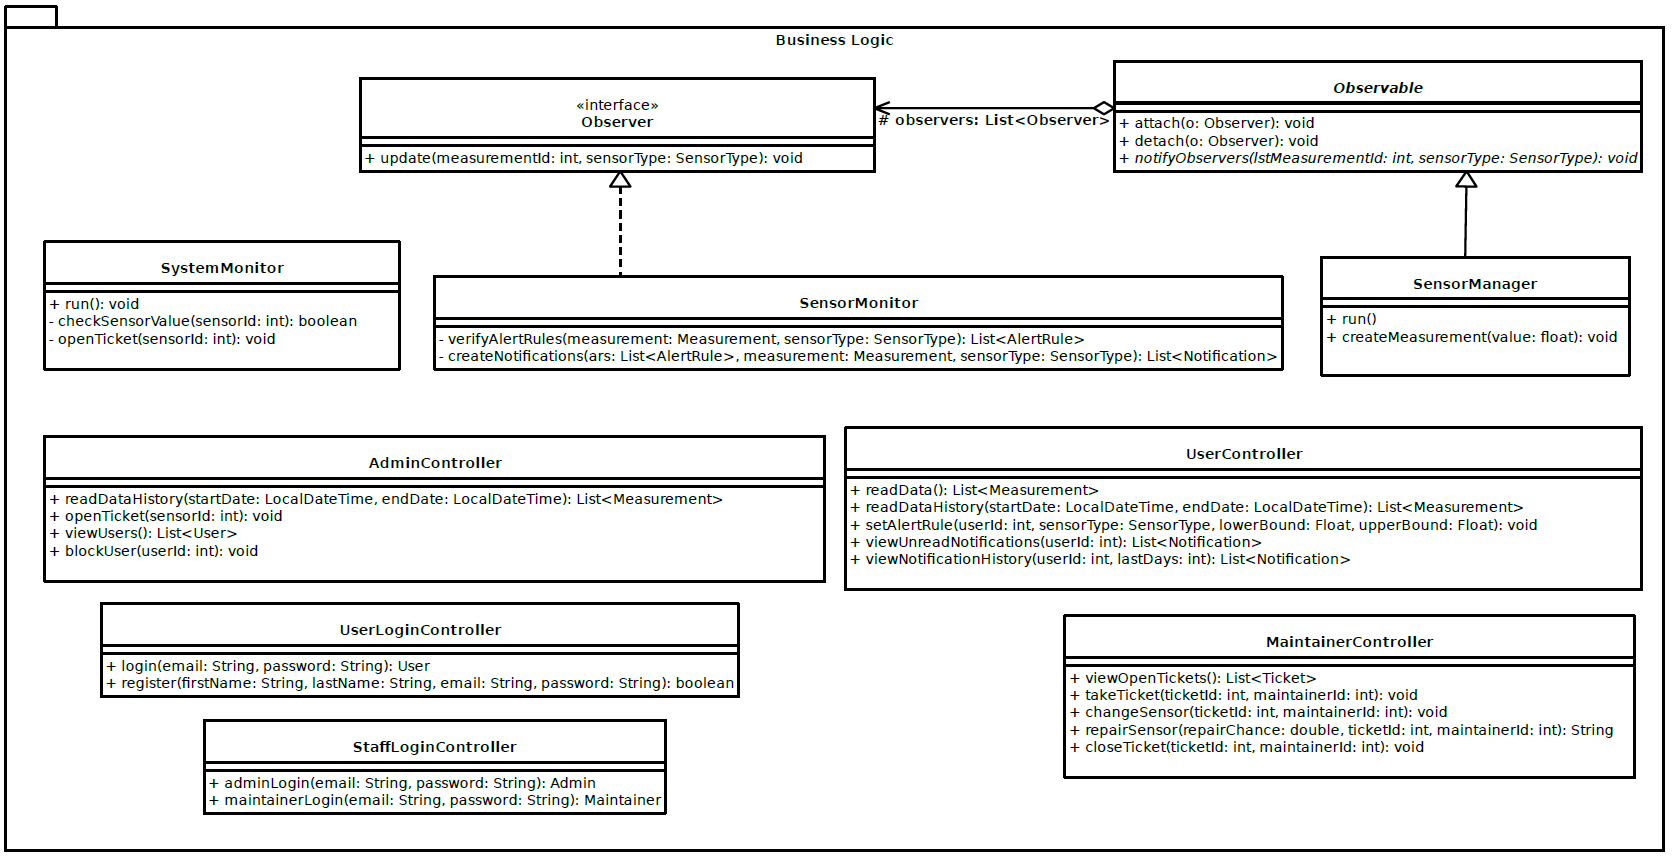
\includegraphics[width=0.95\textwidth]{Images/business_logic}
		\caption{Class Diagram Business Logic}
		\label{fig:business_logic}
	\end{figure}

	\subsubsection{ORM}
	Contiene un oggetto nameClassDAO per ogni classe del domain model presente nel db di sistema. \texttt{ConnectionManager} è la classe che si occupa di erogare e chiudere la connessione al db.
	\begin{figure}[H]
		\centering
		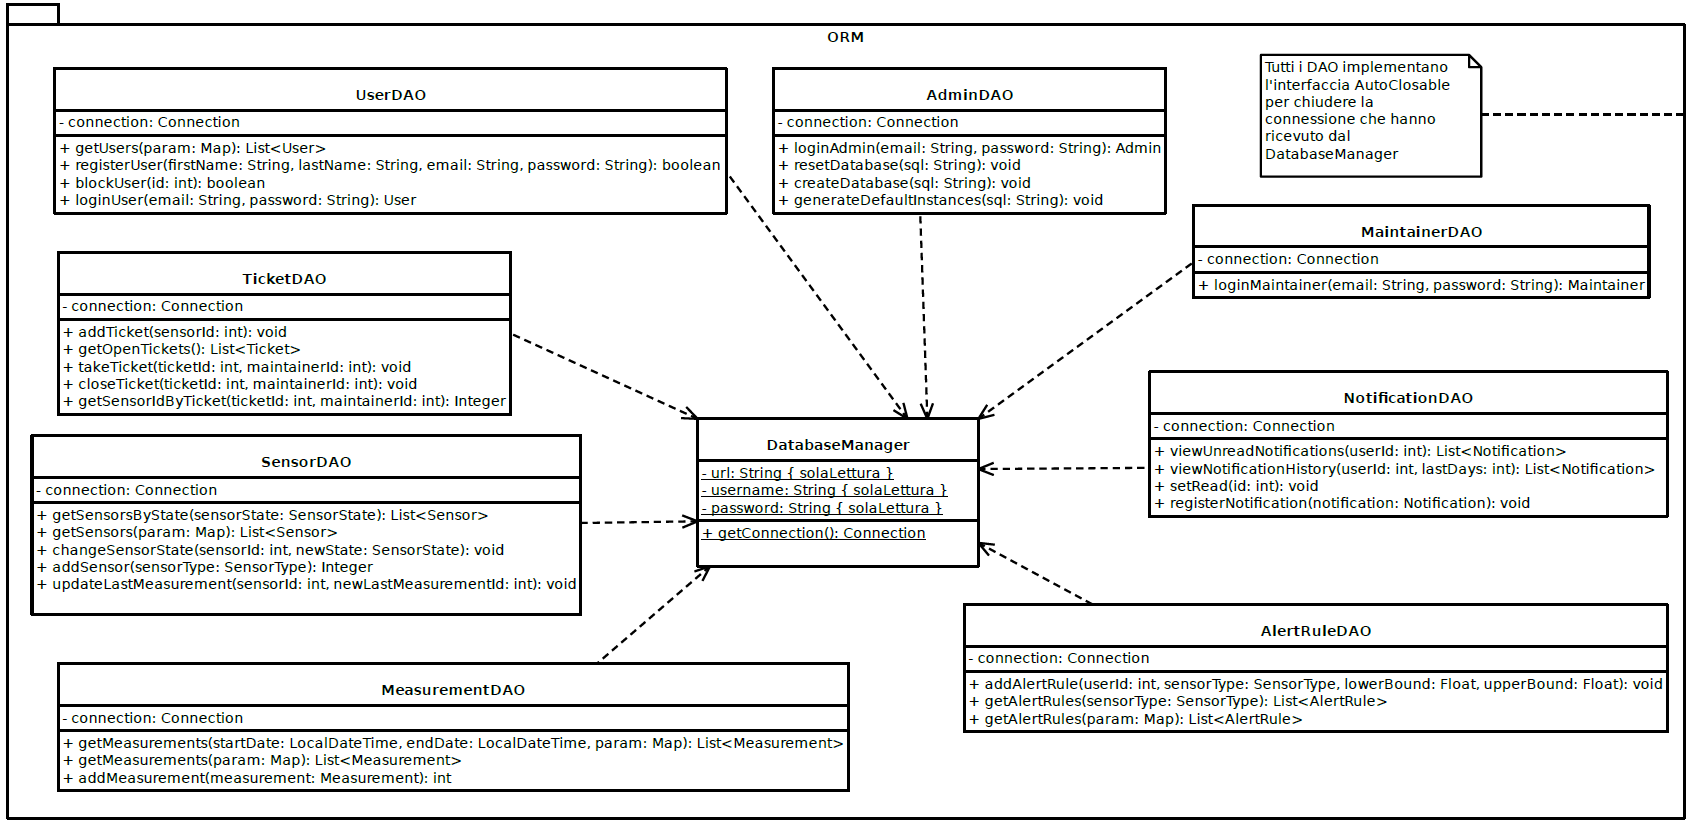
\includegraphics[width=0.95\textwidth]{Images/ORM}
		\caption{Class Diagram ORM}
		\label{fig:ORM}
	\end{figure}

	\subsection{Relationship Model}
	\begin{figure}[H]
		\centering
		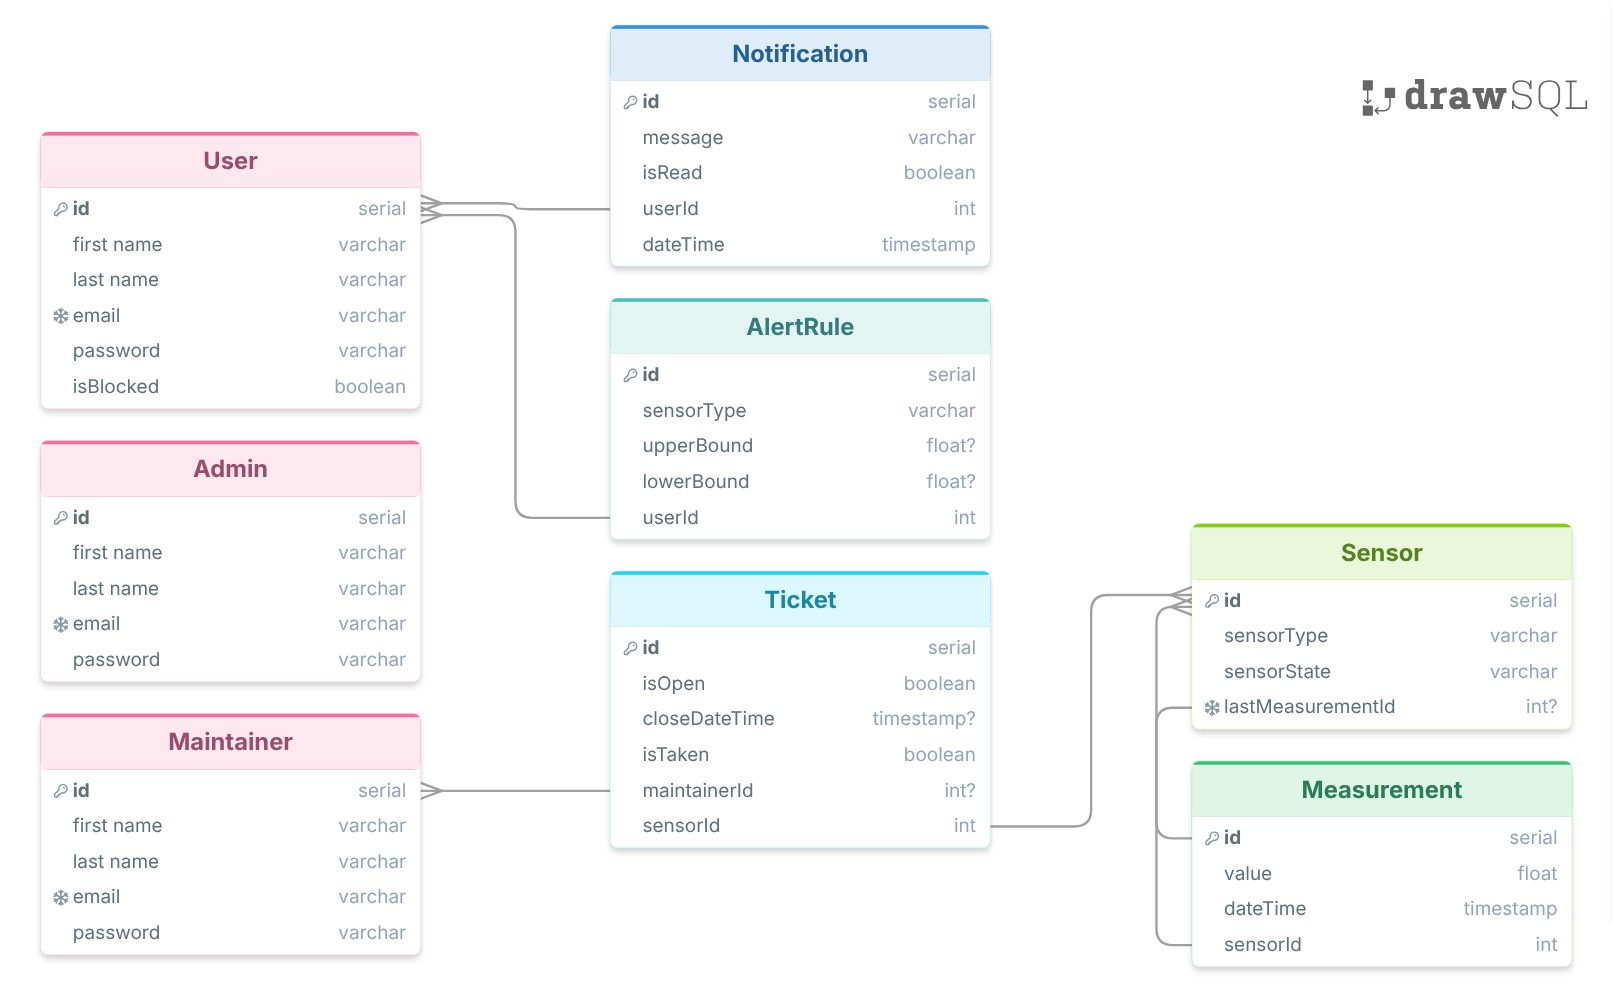
\includegraphics[width=0.95\textwidth]{Images/relational_scheme}
		\caption{ER Diagram}
		\label{fig:Class_ER_Diagram}
	\end{figure}



	NOTA: La tebella AlertRule è inoltre dotata dei seguenti vincoli affinché si mantenga la logica dall'AlertRule stessa:

	\begin{lstlisting}[style=stileSQL]
CREATE TABLE IF NOT EXISTS "AlertRule"
(
    id         SERIAL PRIMARY KEY,
    sensorType VARCHAR(15) NOT NULL,
    lowerBound FLOAT,
    upperBound FLOAT,
    userId INT NOT NULL,
    FOREIGN KEY (userId) REFERENCES "User" (id),
    CONSTRAINT atLeastOneBound CHECK ( lowerBound IS NOT NULL OR upperBound IS NOT NULL ),
    CONSTRAINT rightBoundOrder CHECK ( lowerBound < upperBound )
);
	\end{lstlisting}
	\newline
	Inoltre, a causa della \textbf{relazione circolare} che c'è tra le tabelle Sensor e Measurement, si è reso necessario aggiungere questo controllo:
	\begin{lstlisting}[style = stileSQL]
    ALTER TABLE "Measurement"
    ADD CONSTRAINT fk_sensorId
    FOREIGN KEY (sensorId) REFERENCES "Sensor" (id);
	\end{lstlisting}
	Infatti, una relazione circolare introduce il problema "È nato prima l'uovo o la gallina?", in questo caso per noi è nata prima la tabella Sensor. L'attributo lastMeasurementId potrà essere inizializzato anche in un secondo momento.
	\newline
	Si è reso infine necessario aggiungere anche il suguente controllo:
	\begin{lstlisting}[style = stileSQL]
    CREATE UNIQUE INDEX unique_open_ticket_per_sensor
    ON "Ticket (sensorId)
    WHERE (usOpen = TRUE);
	\end{lstlisting}
	Per un sensore guasto infatti non possono e non devono esserci \textbf{più ticket aperti}.






	\subsection{Mock-ups} % da implementare
	\subsection{Navigation Diagram} % da implementare
	Di seguito è riportato il diagramma di navigazione dell'interfaccia a riga di comando implementata.
	\begin{itemize}
		\item \textbf{Weather station}: La home page. Si sceglie se autenticarsi come utenti o come personale.
		\item \textbf{Dashboard User}: Se si esegue il login come utenti si ha accesso alla lettura dei dati, all'impostazione delle alert rule personalizzate e alla lettura delle notifiche non lette. la lettura dello storico dei dati e dello storico notifiche è gestita mediante una richiesta y/n.
		\item \textbf{Dashboard Admin}: Può visualizzare tutti gli utenti e può leggere lo storico delle misurazioni. Mediante sempre una richiesta y/n sarà chiesto se si desidera bloccare un utente oppure aprire un ticket per un sensore.
		\item \textbf{Dashboard Maintainer}: Visualizza ticket aperti, quindi con richiesta y/n si decide se prenderne uno o meno. Può anche riparare il sensore e chiudere il ticket.
	\end{itemize}
	\begin{figure}[H]
		\centering
		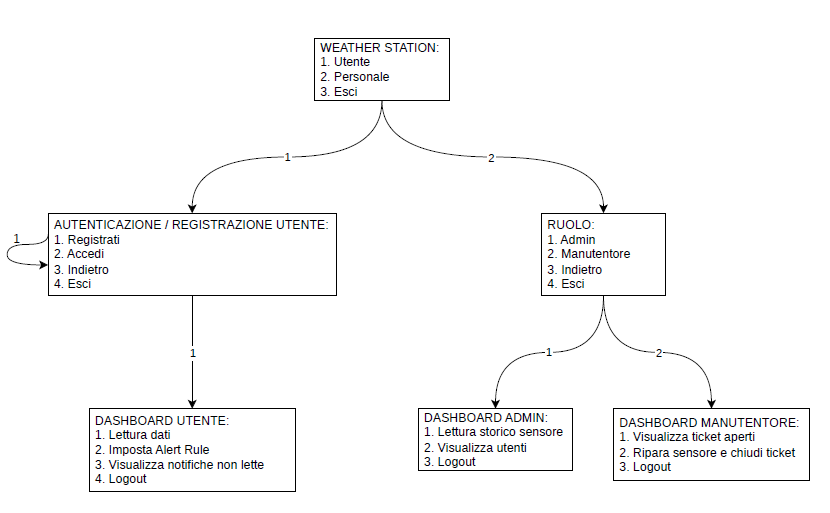
\includegraphics[width=0.95\textwidth]{Images/navigation_diagram}
		\caption{Navigation Diagram}
		\label{fig:navigation_diagram}
	\end{figure}

	\section{Implementazione}
	\subsection{Domain Model}
	\subsubsection{SystemUser}
	Classe astratta che identifica un generico utilizzatore del software. Più nello specifico, è colui che può eseguire un'operazione di login mediante \texttt{email e password}.
	\begin{itemize}
		\item \textbf{User}: Il cliente che usufruisce del servizio come tale. Può leggere le ultime misurazioni, come può leggere lo storico delle misurazioni e può anche creare delle \textbf{alert rules} personalizzate.
		\item \textbf{Admin}: L'amministratore del sistema, nonché la figura con i privilegi più elevati. Può bloccare gli utenti e può aprire manualmente un ticket di manutenzione se, in seguito ad una lettura dei dati da lui eseguita, risultano essere presenti dei valori anomali nei vari sensori, il sensore in questione sarà da lui settato nello stato \texttt{SensorState.FAULTY}.
		\item \textbf{Maintainer}: La figura che può acquisire i ticket di manutenzione, quindi intervenire sui sensori segnalati. Se un sensore viene riparato lo resetta nello stato \texttt{SensorState.ACTIVE}, altrimenti ne aggiungerà uno nuovo impostando permanentemente a \texttt{SensorState.DEACTIVATED} quello guasto.
	\end{itemize}
	\subsubsection{Notification}
	Classe che rappresenta l'oggetto che sarà inviato all'User la cui alert rule è appena stata violata dalle nuove misurazioni. Tra i campi, possiede il flag \texttt{isRead} che, finché sarà \texttt{false}, farà sì che la notifica in questione appaia all'utente nel contenitore delle notifiche non lette.
	\subsubsection{Measurement}
	Classe che identifica una misurazione di un sensore. Sarà quindi specificato l'id del sensore da cui è stata eseguita e il valore della misurazione. Per sapere quale sia la grandezza fisica misurata è necessario accedere alla tabella dei sensori mediante il campo \texttt{sensorId}. ATTENZIONE: le misurazioni potrebbero riportare valori sballati a causa di guasti ai sensori.
	\subsubsection{Ticket}
	Classe che identifica il ticket di segnalazione. Sarà riferito a uno specifico sensore mediante il campo \texttt{sensorId}. Possiede il flag \texttt{isTaken} e il campo \texttt{maintainerId} che, finché saranno rispettivamente false e null, faranno sì che un maintainer possa acquisire tale ticket. Una volta fatto ciò, tale flag sarà settato a true e il campo maintainerId sarà compilato. Il flag \texttt{isOpen} invece resterà true finché il sensore guasto non sarà o riattivato o disattivato e quindi sostituito.
	\subsubsection{Sensor}
	Classe che definisce gli strumenti di misurazione. La classe in sé è astratta ed è implementata in 4 tipi diversi di sensore: \texttt{TemperatureSensor}, \texttt{PressureSensor}, \texttt{WindSensor}, \texttt{HumiditySensor}. Nessuno di questi in realtà introduce nuovi attributi, ciò che li contraddistingue è la diversa implementazione del metodo \texttt{measure()}.

	\subsubsection{Enumerazioni}
	Sono presenti due classi che introducono due diverse enumerazioni:
	\begin{itemize}
		\item \textbf{SensorState}: assume i valori \texttt{ACTIVE, FAULTY, DEACTIVATED}, che rispettivamente rappresentano un sensore in attività regolare, un sensore che è stato contrassegnato come guasto o dall'Admin o dal SystemMonitor, un sensore che è stato permanentemente disattivato da un Maintainer.
		\item \textbf{SensorType}: assume i valori \texttt{TEMPERATURE, PRESSURE, WIND, HUMIDITY}, tali campi sono usati non soltanto all'interno dei sensori, ma anche all'interno delle AlertRule.
	\end{itemize}

	\subsection{Business Logic}
	Le classi di questo package hanno lo scopo di fornire i metodi con cui le varie entità possono interagire col software. In pratica implementano gli Use Cases dei nostri Use Case Diagrams. La caratteristica trasversale di tutte le classi di questo package è che sfruttano i metodi dell'ORM per \textbf{accedere indirettamente} al db. Sarà infatti compito delle classi del package ORM implementare le query richieste.
	\subsubsection{AdminDatabaseController}
	Classe usata principalmente nel testing che ha i metodi per creare la base dati, creare le istanze di default e resettare a zero il database. I metodi della classe altro non fanno che leggere i file della cartella Resources, quindi eseguire il codice in essi contenuto. NOTA: questa è l'unica classe che fa eccezione alla descrizione generale del paragrafo precendente, infatti non sono presenti oggetti DAO.
	\subsubsection{AdminController}
	Classe che implementa i metodi \texttt{readDataHistory(...)}, con la possibilità di leggere i dati relativi o a un sensore specifico o a tutti i sensori, \texttt{viewUsers()} per vedere tutti gli utenti iscritti e \texttt{blockUser(int userId)} per bloccare un determinato utente. Infine \texttt{openTicket(int sensorId)} per aprire manualmente un ticket per un relativo sensore. In merito a quest'ultimo.
	\subsubsection{MaintainerController}
	Troviamo i metodi \texttt{viewOpenTickets(), takeTicket(), closeTicket()} che permettono di selezionare un ticket disponibile, quindi acquisirlo se non è già stato preso. La chiusura avverrà solo in seguito alla riparazione o sostituzione di un sensore, ad opera rispettivamente delle funzioni \texttt{repairSensor(Double reapairChance, int ticketId) e changeSensor(int ticketId)}. Le funzioni sono simulate probabilisticamente mediante la variabile repairChance. NOTA: in alcune di queste funzioni è necessario passare il maintainerId, tale compito è attribuito al Main che salva in memoria il maintainer attualmente loggato (quindi ha accesso al suo id).
	\subsubsection{SystemMonitor}
	Il SystemMonitor è un thread parallelo al Main il cui metodo \texttt{run()} (opportunamente sovrascritto dalla classe base Thread) svolge in automatico la funzione di controllo del valore registrato dai sensori mediante la funzione \texttt{checkSensorValues(int sensorId)}, qualora non risultasse ok (output false) il thread aprirà un ticket per tale sensore. Nel paragrafo successivo sarà detto qualcosa in più sulla sincronizzazione tra i thread SystemMonitor e SensorManager.
	\subsubsection{SensorManager – D. P. Observer}
	Il SensorManager è l'altro thread menzionato nel paragrafo del System Monitor. Questa classe \texttt{estende la classe astratta Observable} e, assieme a SensorMonitor, va a implementare il design pattern observer del software. Il suo \texttt{run()} è l'unico metodo del software che aziona i sensori, consentendo loro di misurare tramite il metodo \texttt{measure()}. La misura viene poi opportunamente salvata nel database. Il thread invoca il metodo \texttt{notifyObservers(...)} per propagare l'Id della misurazione e il tipo di sensore al SensorMonitor, cosicché questo possa eseguire a sua volta il suo \texttt{update(...)} (vedi paragrafo successivo) . La sincronizzazione tra questi due thread è realizzata mediante la classe \textbf{DatabaseMutex}, essa in realtà contiene solo un \texttt{Semaphore(1)} come attributo statico. I due thread prima di agire devono eseguire l'acquire di tale mutex. La logica è che nel mentre i sensori vengono controllati non possano eseguire ulteriori misurazioni, che sarebbero a loro volta errate in caso di guasto.


	\subsubsection{SensorMonitor – D. P. Observer}
	Classe che \texttt{implementa l'interfaccia Observer}. Il suo metodo \texttt{update(...)} si occupa di creare e inserire nel database le notifiche scaturite in seguito alla violazione di un bound di una AlertRule per una certa grandezza fisica. La verifica è effettuata mediante il metodo \texttt{verifyAlertRule(...)}.

	\subsubsection{UserController}
	Classe che definisce cosa un cliente iscritto e non bloccato può fare. Può leggere le misurazioni con \texttt{readData(...) e readDataHistory(...)}. Può settare una nuova alert rule personalizzata mediante \texttt{setAlertRule(...)}, un appunto che si può fare in merito a tale funzione è che è stata realizzata in modo da consentire di imporre sia un intervallo di tolleranza che solamente un limite inferiore o superiore per le misurazioni. Ad esempio, si può imporre di essere avvisati sia che la temperatura T sia solo $T<20$ che sia solo $T>30$ o che sia l'uno o l'altro. Il cliente può inoltre leggere le notifiche non lette o direttamente lo storico delle notifiche con i metodi \texttt{viewUnreadNotification(...) e viewNotificationHistory(...)}.
	\subsubsection{StaffLoginController}
	Classe che contiene i metodi \texttt{adminLogin(String email, String password) e maintainerLogin(String email, String password)}, i login dello staff appunto. Si rende evidente che questo software adotta la procedura di login mediante le credenziali email e password.
	\subsubsection{UserLoginController}
	Classe che contiene i metodi \texttt{login(String email, String password) e register(...)}. Questi sono solo per lo User.

	\subsection{ORM}
	\subsubsection{DatabaseManager e interfaccia AutoClosable}
	DatabaseManager è la classe che si occupa di fornire la connessione al nostro database. La logica di connessione al database è centralizzata in questa unica classe, infatti i parametri d'accesso sono tenuti solamente qui. La connessione è restituita mediante il metodo \texttt{getConnection(...)} come oggetto di tipo Connection. Nei vari metodiDAO la Connection sarà chiusa in automatico al termine del codice di ognuno di essi grazie all'implementazione dell'interfaccia AutoClosable, in merito a ciò può notare come ogni oggetto DAO sia inizializzato nel blocco resources dei vari try al fine di consentire il corretto funzionamento di tale maccanica.
	\subsubsection{AdminDAO e MaintainerDAO}
	Contengono il metodo \texttt{login(...)} per ottenere la relativa istanza dal db. La classe AdminDAO contiene inoltre i metodi per creare e resettare il db, nonché inizializzarlo con le istanze di default.
	\subsubsection{AlertRuleDAO}
	Ha il metodo \texttt{addAlertRule(...)} per inserire nel db una nuova alert rule e il metodo \texttt{getAlertRule(...)} per eseguire una select che può agire sulla base o di una \texttt{Map<String, Object>} o su una variabile \texttt{SensorType} in ingresso.
	\subsubsection{MeasurementDAO}
	Similmente alla precedente AlertRuleDAO, c'è un metodo \texttt{addMeasurement(...)} per l'inserimento di nuove misure e un metodo \texttt{getMeasurement(...)} che può prendere in ingresso o soltanto la solita generica \texttt{Map<String, Object>} oppure, oltre a questa, anche un intervallo di date che definiranno l'intervallo temporale di cui si desidera leggere le misure effettuate dai sensori.
	\subsubsection{NotificationDAO}
	Qui è presente il metodo \texttt{registerNotification(...)} che inserisce una nuova notifca nel db. Ci sono i metodi \texttt{viewUnreadNotification(...), viewNotificationHistory(int userId, int lastDays)} che filtrano la lettura delle notifiche rispettivamente per avvenuta lettura o meno e se sono risalenti a non più di \texttt{lastDays} giorni fa. In seguito alla chiamata di \texttt{viewUnreadNotification(...)} da parte di UserController, ci sarà anche una chiamata al metodo \texttt{setRead()} che setterà a true il campo isRead della tupla relativa alla notifica appena letta.
	\subsubsection{SensorDAO}
	Ci sono due metodi per eseguire una select dei sensori: il metodo \texttt{getSensors(Map<String. Object> map)} e \texttt{getSensorByState(SensorState sensorState)}. A causa della gerarchia ereditaria, con conseguente presenza di diversi costruttori per ogni sensore, si è reso necessario uno switch-cases a seconda del tipo di sensore. Vi è poi il metodo \texttt{changeSensorState(int sensorID, SensorState newState)} che si occupa di modificare lo status di un sensore in seguito a qualche evento: l'apertura di un ticket fa sì che un sensorState venga settato a FAULTY, la riparazione lo fa tornare nello stato ACTIVE, mentre la sostituzione lo rende permanentemente DEACTIVATED. L'inserimento di un nuovo sensore è consentito dal metodo \texttt{addSensor(...)}. Non esiste un metodo per la rimozione dei sensori: i sensori DEACTIVATED rimangono nel database come tali al fine non creare tuple orfane all'interno del databse stesso, l'id del sensore è infatti chiave esterna di alcune tabelle. Infine abbiamo il metodo \texttt{updateLastMeasurement(...)} che modifica l'id dell'ultima misura effettuata da un sensore, tale metodo è ovviamente chiamato al momento della misura del sensore stesso.
	\begin{lstlisting}
    try (ResultSet resultSet = statement.executeQuery()) {
                while (resultSet.next()) {
                    int id = resultSet.getInt("id");
                    Integer lastMeas = (Integer) resultSet.getObject("lastMeasurementId");
                    SensorType myType = SensorType.valueOf(resultSet.getString("sensorType"));
                    SensorState myState = SensorState.valueOf(resultSet.getString("sensorState"));

                    Sensor sensor = switch (myType) {
                        case HUMIDITY -> new HumiditySensor(id, lastMeas, myType, myState);
                        case WIND -> new WindSensor(id, lastMeas, myType, myState);
                        case TEMPERATURE -> new TemperatureSensor(id, lastMeas, myType, myState);
                        case PRESSURE -> new PressureSensor(id, lastMeas, myType, myState);
                    };

                    sensors.add(sensor);
                }
            } catch (SQLException e) {
                System.err.println("Errore durante la query del recupero dei sensori guasti: " + e.getMessage());
                e.getStackTrace();
            }
	\end{lstlisting}
	\subsubsection{TicketDAO}
	Per inserire nuovi ticket c'è \texttt{addTicket(...)}, in ordine poi abbiamo \texttt{getOpenTicket(), takeTicket(...), closeTicket(...)} per le rispettive azioni. Vi è inoltre il metodo \texttt{getSensorIdByTicket(...)}, usato nel MaintainerController, questo perché tramite un ticket è possibile risalire al sensore guasto, vedi schema relazionale.
	\subsubsection{UserDAO}
	Il metodo \texttt{getUsers(Map<String, Object> map)} esegue una select degli utenti col solito criterio della mappa. Ci sono poi i metodi per la registrazione e il login e il metodo \texttt{blockUser(int userId)} per settare a true il campo isBlocked nella tabella User.

	\section{Testing}
	In quest'ultima sezione sono presenti snippet di codice che mostrano come sono stati realizzati alcuni test.
	\subsection{Business Logic Test}
	\subsubsection{AdminControllerTest}
	\begin{lstlisting}
      @Test
    void blockUser() {
        ArrayList<User> users = new ArrayList<>();
        try (UserDAO userDAO = new UserDAO()) {
            users = userDAO.getUsers(Map.of("id", 2));
            assertEquals(1, users.size()); //Verifica che abbia prelevato un solo utente
        } catch (SQLException e) {
            System.err.println("Error in userDAO: " + e.getMessage());
        }
        User u1 = users.getFirst();
        adminController.blockUser(u1.getId());
        try (UserDAO userDAO = new UserDAO()) {
            users = userDAO.getUsers(Map.of("id", 2));
            assertEquals(1, users.size());
        } catch (SQLException e) {
            System.err.println("Error in userDAO: " + e.getMessage());
        }
        User actualUser = users.getFirst();   //Adesso dovrebbe essere bloccato
        assertTrue(actualUser.isBlocked());

        adminController.blockUser(u1.getId());//Provo a bloccare nuovamente lo stesso utente per vedere cosa succede
        try (UserDAO userDAO = new UserDAO()) {
            users = userDAO.getUsers(Map.of("id", 2));
            assertEquals(1, users.size()); //Verifica che abbia prelevato un solo utente
        } catch (SQLException e) {
            System.err.println("Error in userDAO: " + e.getMessage());
        }
        actualUser = users.getFirst();   //Ora dovrebbe comunque essere bloccato
        assertTrue(actualUser.isBlocked());
    }

    @Test
    void openTicket() {
        Ticket expectedTicket = new Ticket(1, 2, null, true, false, null);
        Ticket actualTicket;
        try (TicketDAO ticketDAO = new TicketDAO()) {
            adminController.openTicket(2);
            actualTicket = ticketDAO.getOpenTickets().getFirst();
            assertEquals(expectedTicket, actualTicket);
            assertThrows(SQLException.class, () -> adminController.openTicket(2)); //non puo' inserire un altro ticket ne esite gia' uno aperto
        } catch (SQLException e) {
            System.err.println("Error in ticketDAO: " + e.getMessage());
        }
    }
	\end{lstlisting}
	\subsubsection{MaintainerControllerTest}
	\begin{lstlisting}
      @Test
    void takeTicket_success() {
        try (TicketDAO ticketDAO = new TicketDAO()){
            ticketDAO.addTicket(1);
        }catch (SQLException e){
            System.err.println(e.getMessage());
        }
        assertDoesNotThrow(() -> maintainerController.takeTicket(1, 1));
    }

    @Test
    void takeTicket_notFound() {
        try (TicketDAO ticketDAO = new TicketDAO()){
            ticketDAO.addTicket(1);
        }catch (SQLException e){
            System.err.println(e.getMessage());
        }
        assertThrows(SQLException.class ,() -> maintainerController.takeTicket(2, 1));
    }

    @Test
    void takeTicket_alreadyTaken() {
        try (TicketDAO ticketDAO = new TicketDAO()){
            ticketDAO.addTicket(1);
        }catch (SQLException e){
            System.err.println(e.getMessage());
        }
        try {
            maintainerController.takeTicket(1, 1);
        } catch (SQLException e) {
           e.getStackTrace();
        }

        assertThrows(SQLException.class ,() -> maintainerController.takeTicket(1, 1));
    }

    @Test
    void closeTicket_success() {
        try (TicketDAO ticketDAO = new TicketDAO()){
            ticketDAO.addTicket(1);
            maintainerController.takeTicket(1, 1);
            assertDoesNotThrow(() -> maintainerController.closeTicket(1, 1));
        }catch (SQLException e){
            System.err.println("Test viewOpenTicket exception");
        }
    }

    @Test
    void closeTicket_alreadyClosed() {
        try (TicketDAO ticketDAO = new TicketDAO()) {
            ticketDAO.addTicket(1);
            maintainerController.takeTicket(1, 1);
            maintainerController.closeTicket(1, 1);
            assertThrows(SQLException.class, () -> maintainerController.takeTicket(1, 1));
        } catch (SQLException e) {
            System.err.println(e.getMessage());
        }
    }

    @Test
    void closeTicket_notHisTicket() {
        try (TicketDAO ticketDAO = new TicketDAO()) {
            ticketDAO.addTicket(1);
            ticketDAO.takeTicket(1, 2);
            assertThrows(SQLException.class, () -> maintainerController.closeTicket(1, 1));
        } catch (SQLException e) {
            System.err.println(e.getMessage());
        }
    }

    @Test
    void repairSensor() {
        double repairChance;
        boolean fixed = false, changed = false;
        try (SensorDAO sensorDAO = new SensorDAO(); TicketDAO ticketDAO = new TicketDAO()) {
            while (!fixed || !changed) {

                repairChance = Math.random();
                ticketDAO.addTicket(1);
                ticketDAO.takeTicket(1, 1);

                //forziamo il sensore a diventare guasto
                Map<String, Object> map = new HashMap<>();
                map.put("id", 1);
                ArrayList<Sensor> target = sensorDAO.getSensors(map);
                target.getFirst().sensorStateToFaulty();

                String result = maintainerController.repairSensor(repairChance, 1, 1);

                if (repairChance < 0.88) {
                    target = sensorDAO.getSensors(map);
                    assertEquals(SensorState.ACTIVE, target.getFirst().getSensorState());
                    assertThrows(SQLException.class, () -> ticketDAO.closeTicket(1, 1));   //per verificare che il ticket sia stato chiuso da repairSensor()
                    assertEquals("sensore_riparato", result);
                    fixed = true;
                } else {
                    assertEquals("sensore_sostituito", result);
                    changed = true;
                }
                adminDatabaseController = new AdminDatabaseController();
                try{
                    adminDatabaseController.resetDatabase();
                    adminDatabaseController.createDatabase();
                    adminDatabaseController.defaultInstances();
                }catch (SQLException e){
                    System.out.println("Errore durante il reset del database");
                }
            }
        } catch (SQLException e) {
            System.err.println("Test repairSensor exception");
            e.printStackTrace();
        }

    }
	\end{lstlisting}
	NOTA: quest'ultimo è stato testat a tentativi vista la aleatorietà dei metodi testati
	\subsubsection{UserLoginControllerTest}
	\begin{lstlisting}
      @DisplayName("User presente e credenziali esatte")
    @Test
    void login_success() {
        User user = new User(2, "Roberto", "Chiesi", "robertochiesi@test.it", false);
        assertEquals(user, userLoginController.login("robertochiesi@test.it", "123"));
    }

    @DisplayName("User presente, ma credenziali errate")
    @Test
    void login_fail1() {
        assertNull(userLoginController.login("robertochiesi@test.it", "abc"));
        assertNull(userLoginController.login("robertochiesi@email.it", "123"));
    }

    @DisplayName("User non presente nel database")
    @Test
    void login_fail2() {
        assertNull(userLoginController.login("yuribartoletti@test.it", "123"));
    }

    @DisplayName("User presente, ma bloccato")
    @Test
    void login_fail3() {
        assertNull(userLoginController.login("samuelezanieri@test.it", "123"));
    }

    @DisplayName("Registrazione con successo")
    @Test
    void register_success() {
        assertTrue(userLoginController.register("Luke", "Skywalker", "lukeskywalker@test.it", "123"));
        assertNotNull(userLoginController.login("lukeskywalker@test.it", "123"));
    }

    @DisplayName("User gia' registrato")
    @Test
    void register_fail1() {
        assertFalse(userLoginController.register("Samuele", "Skywalker", "samuelezanieri@test.it", "123"));
    }

    @DisplayName("Email o password troppo lunghe")
    @Test
    void register_fail2() {
        StringBuilder stringBuilder = new StringBuilder(55);
        stringBuilder.repeat("a", Math.max(0, stringBuilder.capacity()));
        String email = stringBuilder.toString();
        assertFalse(userLoginController.register("Luke","Skywalker", email, "123"));
        stringBuilder = new StringBuilder(260);
        stringBuilder.repeat("a", Math.max(0, stringBuilder.capacity()));
        String password = stringBuilder.toString();
        assertFalse(userLoginController.register("Luke", "Skywalker", "lukeskywalker@test.it", password));
    }
	\end{lstlisting}
	La logica dei testi della classe StaffLoginController è fondamentalmente la solita, dunque è stata omessa in questa relazione


	\subsubsection{UserControllerTest}
	\begin{lstlisting}
      @Test
    void setAlertRule() {
        userController.setAlertRule(1, SensorType.TEMPERATURE, 11f, 51f);
        userController.setAlertRule(2, SensorType.WIND, null, 89f);
        userController.setAlertRule(3, SensorType.HUMIDITY, 36f, null);

        ArrayList<AlertRule> comparing = new ArrayList<>();
        ArrayList<AlertRule> results = new ArrayList<>();
        comparing.add(new AlertRule(7, 1, 11f, 51f, SensorType.TEMPERATURE));
        comparing.add(new AlertRule(8, 2, null, 89f, SensorType.WIND));
        comparing.add(new AlertRule(9, 3, 36f, null, SensorType.HUMIDITY));
        try (AlertRuleDAO alertRuleDAO = new AlertRuleDAO()){
            Map<String, Object> map = new HashMap<>();
            map.put("id", 7);
            results.add(alertRuleDAO.getAlertRules(map).getFirst());
            map.clear();
            map.put("id", 8);
            results.add(alertRuleDAO.getAlertRules(map).getFirst());
            map.clear();
            map.put("id", 9);
            results.add(alertRuleDAO.getAlertRules(map).getFirst());

        }catch (SQLException e){
            System.err.println("Error in setAlertRule Test: "+e.getMessage());
        }

        assertIterableEquals(comparing, results);
    }
	\end{lstlisting}
	\subsection{Domain Model}
	\subsubsection{AlertRuleTest}
	\begin{lstlisting}
      @Test
    void isViolatedBy_lowerBoundViolated() {
        Measurement measurement = new Measurement(0, 0, 14f, null);
        assertTrue(alertRule.isViolatedBy(measurement));
    }

    @Test
    void isViolatedBy_upperBoundViolated() {
        Measurement measurement = new Measurement(0, 0, 51f, null);
        assertTrue(alertRule.isViolatedBy(measurement));
    }

    @Test
    void isViolatedBy_valueInRange() {
        Measurement measurement = new Measurement(0, 0, 35f, null);
        assertFalse(alertRule.isViolatedBy(measurement));
    }

    @Test
    void isViolatedBy_valueEqualsLowerBound() {
        Measurement measurement = new Measurement(0, 0, 15f, null);
        assertFalse(alertRule.isViolatedBy(measurement));
    }

    @Test
    void isViolatedBy_valueEqualsUpperBound() {
        Measurement measurement = new Measurement(0, 0, 50f, null);
        assertFalse(alertRule.isViolatedBy(measurement));
    }
	\end{lstlisting}

\end{document}